\chapter{Simple Units and Networks}
\label{ch:simple-units}

\textit{A neural model is defined by its state variables and by the question it is meant to answer. This chapter starts from that principle, then develops the perceptron as the simplest example of classification by weighted summation and thresholding.}

% ============================================================
\section{Why Model?}
\label{sec:why-model}
% ============================================================

A model is useful only relative to a question. It keeps the variables needed to explain or predict a phenomenon and discards the rest. More detail is not automatically better; irrelevant detail hides mechanism.

If the question is spike initiation, the natural variables are conductances, reversal potentials, and gating kinetics. If the question is classification, those variables are the wrong ones; weighted inputs and a decision boundary are enough. The correct abstraction is therefore task-dependent.

Across computational neuroscience, the same biological system can be described at several levels: channel states, membrane voltage, spike times, population activity, or latent behavioral variables. Each upward step coarse-grains the system and trades mechanistic detail for analytic simplicity.

\begin{figure}[h]
\centering
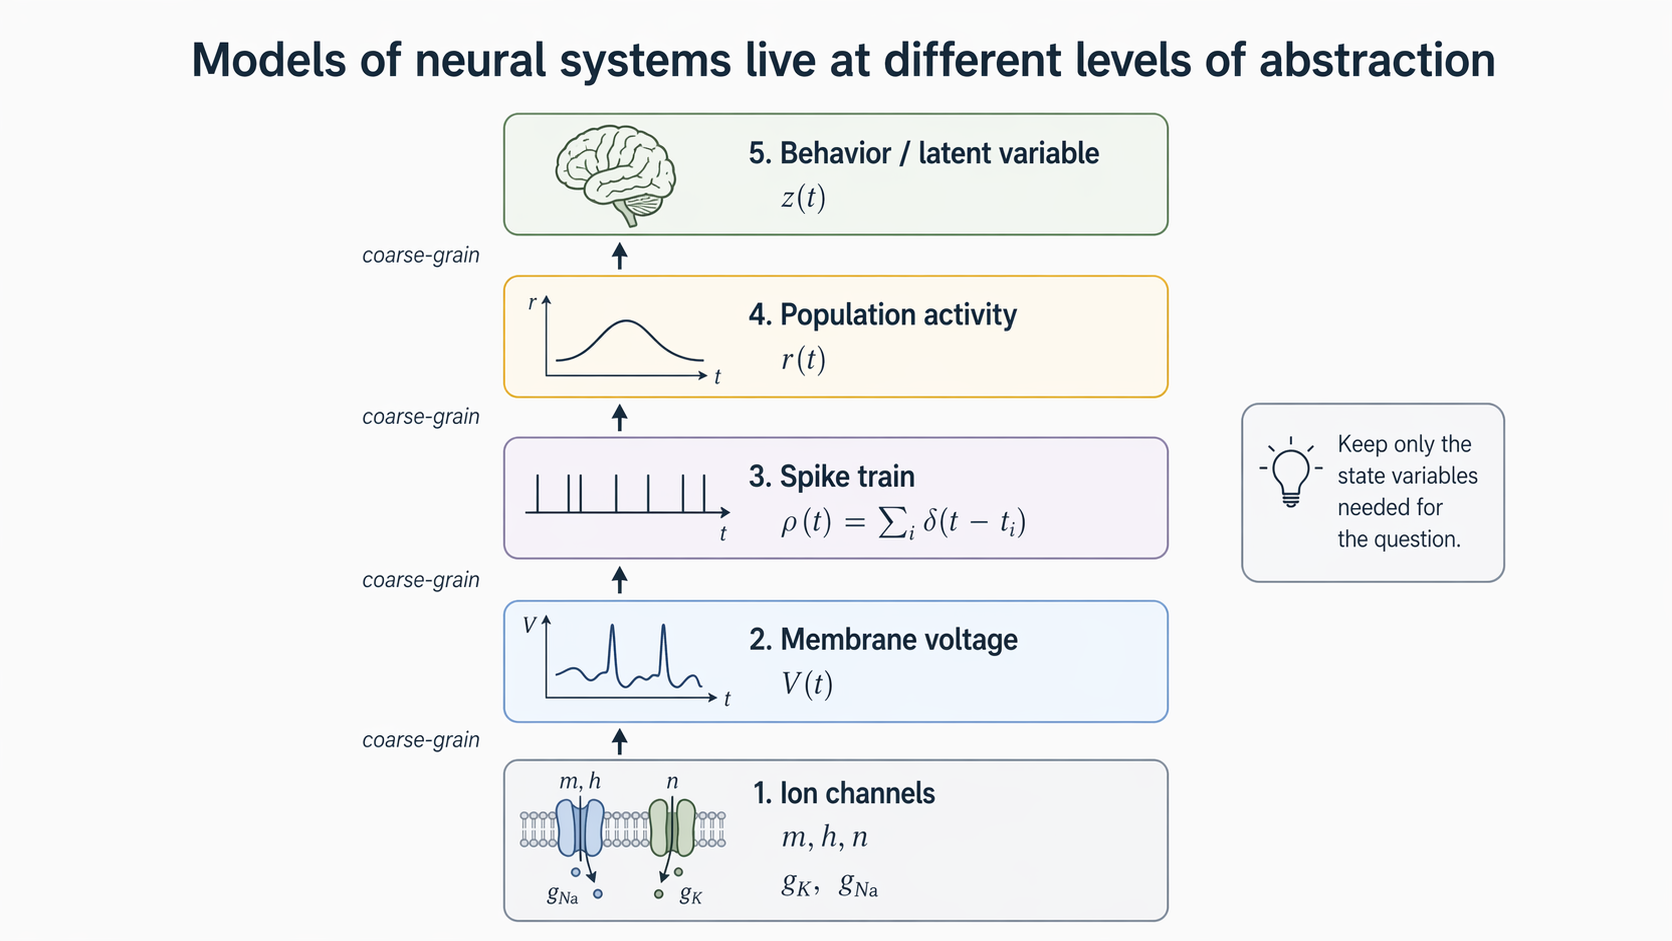
\includegraphics[width=\textwidth]{figures/mns-abstraction-levels.png}
\caption{A modeling hierarchy from channel states to behavior. Each level retains only the state variables needed for the current question and treats the rest as hidden detail.}
\label{fig:modeling-levels}
\end{figure}

This hierarchy prevents a common mistake: asking a model to explain phenomena outside its state description. A point neuron cannot answer a dendritic propagation question, and a rate model cannot explain spike-timing precision without additional structure.

% ============================================================
\section{Classification as a Computational Task}
\label{sec:classification}
% ============================================================

Many things the brain does can be framed as classification\index{classification}: given some sensory input, assign it to a category. Is this object a face or not? Is this sound a vowel or a consonant? Should I move left or right?

Abstractly, we have a feature vector $\vec{x} \in S_x$ and a set of labels $S_y$. Classification means finding a function $f: S_x \to S_y$ that maps inputs to correct labels. The challenge is that the space of possible mappings is enormous. If each input is a binary vector of length $n$, there are $2^n$ possible inputs and $|S_y|^{2^n}$ possible functions. Even for modest $n$, this number is far too large for a lookup table.

The brain solves this problem efficiently. There is evidence that higher cortical areas store something like prototypes---internal representations of typical examples for each category. A new input is compared to these prototypes, and the closest match determines the classification. The question is: what is the simplest mathematical device that can do this?

% ============================================================
\section{The Perceptron}
\label{sec:perceptron}
% ============================================================

The perceptron\index{perceptron} is the simplest model of a neuron that can perform classification. It takes $n$ inputs, computes a weighted sum, and passes the result through a nonlinear function:

\begin{keyequation}[The Perceptron]
\begin{equation}
  y = f\!\Bigl(\sum_{i=1}^{n} w_i x_i - \theta\Bigr)
  \label{eq:perceptron}
\end{equation}
\tcblower
$x_i$: input (firing rate of neuron $i$), \quad
$w_i$: synaptic weight, \quad
$\theta$: threshold, \quad
$f$: transfer function.
\end{keyequation}

\noindent The weighted sum $h = \sum_i w_i x_i$ is called the \emph{activation}\index{activation}. The transfer function $f$ determines the output format. Common choices include the step function (McCulloch--Pitts neuron\index{McCulloch--Pitts neuron}), which outputs $1$ if $h > \theta$ and $0$ otherwise, and smooth alternatives like the sigmoid $f(z) = 1/(1 + e^{-z})$.

What does the perceptron actually compute? Writing the activation in vector notation, $h = \vec{w} \cdot \vec{x}$, we see that it is a \emph{dot product}\index{dot product}. The output is large when the input $\vec{x}$ points in roughly the same direction as the weight vector $\vec{w}$, and small or zero when they point in different directions. The perceptron is, at its core, a similarity detector: it measures how closely the current input matches the pattern stored in the weights.

\subsection{Decision boundaries}

The threshold condition $\vec{w} \cdot \vec{x} = \theta$ defines a \emph{hyperplane}\index{hyperplane} in input space. On one side the perceptron outputs $1$; on the other side it outputs $0$. The weight vector $\vec{w}$ is perpendicular to this hyperplane, and the threshold $\theta$ determines how far the hyperplane sits from the origin.

For a two-class problem, the perceptron divides input space into two half-spaces. Any input falling on the $\vec{w}$ side of the hyperplane is classified as ``yes''; anything on the other side is classified as ``no.'' This geometric picture makes the perceptron's power and limitations immediately clear.

\begin{figure}[h]
\centering
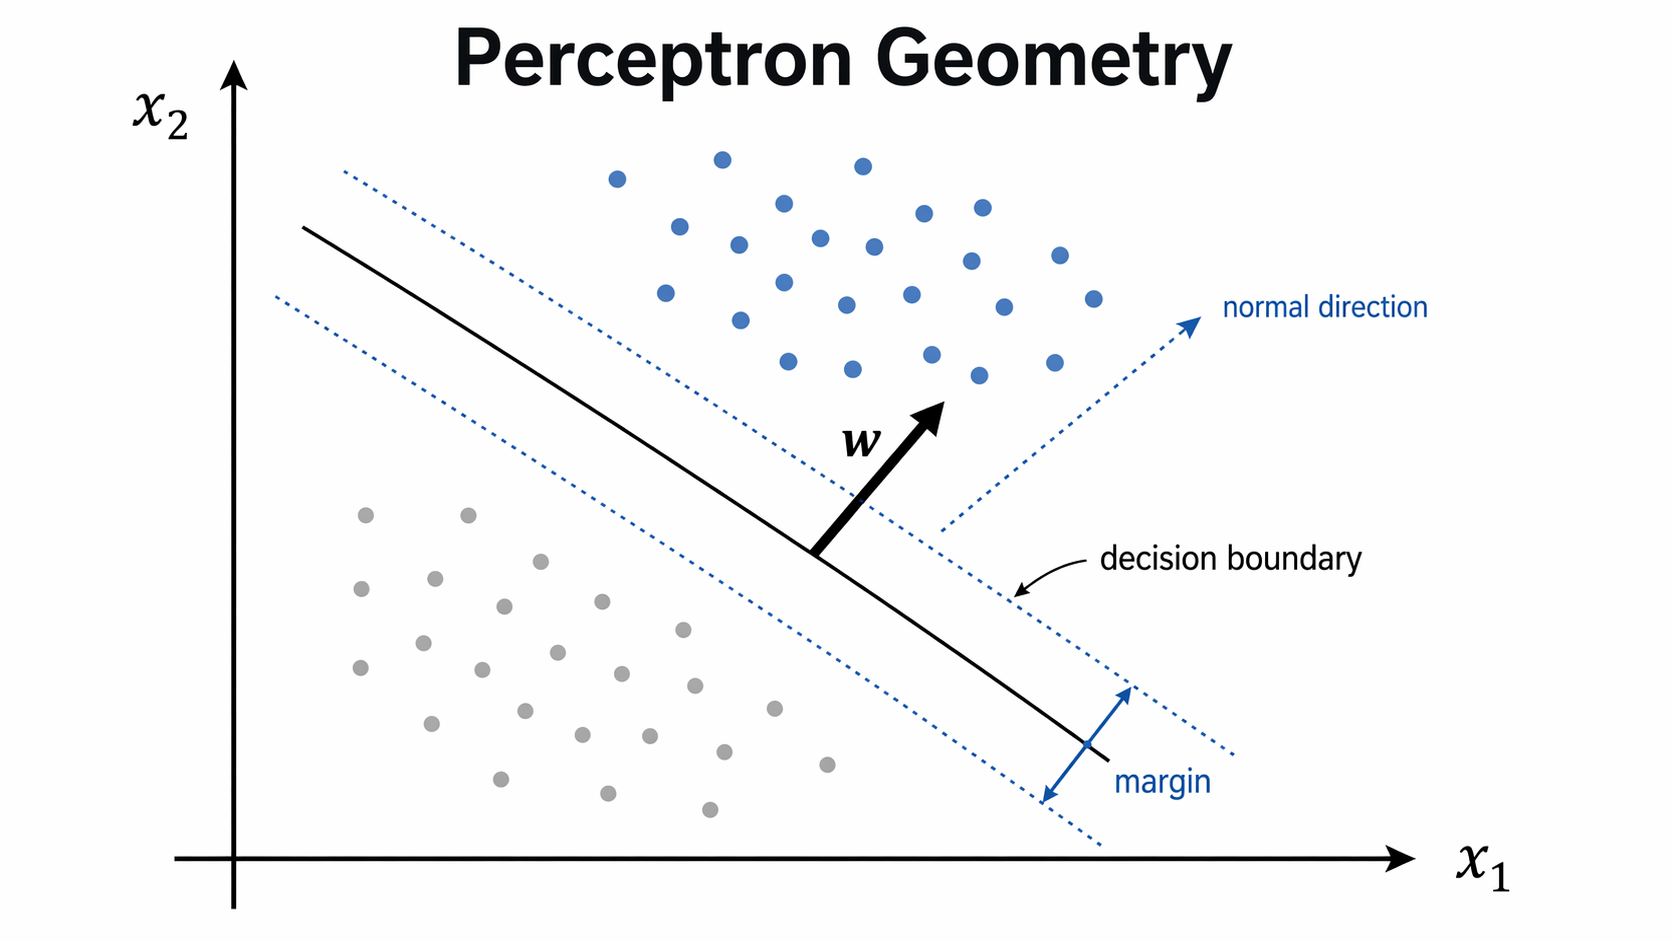
\includegraphics[width=\textwidth]{figures/mns-perceptron-geometry.png}
\caption{Perceptron geometry. The equation $\vec{w}\cdot\vec{x}=\theta$ defines the decision boundary; $\vec{w}$ is normal to that boundary, and the margin measures signed distance from the separating hyperplane.}
\label{fig:perceptron-geometry}
\end{figure}

% ============================================================
\section{Linear Separability}
\label{sec:linear-sep}
% ============================================================

A classification problem is \emph{linearly separable}\index{linear separability} if there exists a hyperplane that correctly separates all inputs of one class from all inputs of the other. The perceptron can solve a problem if and only if it is linearly separable.

Many problems are linearly separable. If two categories of objects differ systematically along some combination of features, a single hyperplane can separate them. But some problems are not. The canonical example is the XOR function: given two binary inputs $x_1, x_2 \in \{0, 1\}$, output $1$ if exactly one input is $1$, and $0$ otherwise. No single line in the $(x_1, x_2)$ plane can separate the $(0,0)$ and $(1,1)$ points (both class $0$) from the $(0,1)$ and $(1,0)$ points (both class $1$). The perceptron fails here.

This is not a minor technicality. It tells us something fundamental: a single neuron with a linear decision boundary cannot represent arbitrary input--output relationships. To go further, we need either more neurons or a different architecture.

% ============================================================
\section{The Dot Product as Similarity}
\label{sec:dot-product}
% ============================================================

The fact that the perceptron computes a dot product deserves emphasis, because this operation appears throughout neuroscience and machine learning. If both $\vec{w}$ and $\vec{x}$ are normalized to unit length, then $\vec{w} \cdot \vec{x} = \cos\alpha$, where $\alpha$ is the angle between them. The dot product is maximal when the two vectors are aligned and zero when they are orthogonal.

This gives a natural interpretation of what the weights represent: the weight vector $\vec{w}$ is a \emph{template}\index{template matching} or prototype. The perceptron fires when the input is sufficiently similar to the template. This is consistent with the neuroscience idea that certain neurons act as feature detectors---cells in inferotemporal cortex, for instance, respond selectively to specific objects or faces. The weight vector of such a neuron encodes its preferred stimulus.

Winner-take-all competition among multiple perceptrons, each with a different weight vector, implements nearest-prototype classification. The input is assigned to the category whose prototype it most closely resembles. This is one of the simplest models of categorical perception.

% ============================================================
\section{Multilayer Networks}
\label{sec:multilayer}
% ============================================================

The limitations of a single perceptron disappear when we stack multiple layers. A \emph{multilayer feedforward network}\index{multilayer network} passes the input through one or more hidden layers before the output. Each hidden unit computes a weighted sum plus nonlinearity, and the outputs of one layer become the inputs to the next.

Why does depth help? Each hidden unit creates its own hyperplane in input space. The combination of many hyperplanes can carve out arbitrarily complex decision regions. A two-layer network with enough hidden units can separate any set of points---it is not limited to linearly separable problems.

This idea is made precise by the \emph{universal approximation theorem}\index{universal approximation theorem}: a feedforward network with a single hidden layer of sufficient width and a non-polynomial activation function can approximate any continuous function on a compact domain to arbitrary accuracy. The key requirement is that the activation function is nonlinear. A network of purely linear units, no matter how deep, can only compute linear functions---the composition of linear maps is still linear.

The intuition is straightforward. Each hidden unit with a nonlinear activation (say, a ReLU\index{ReLU}) creates a ``kink'' in the function along some hyperplane. By rotating, shifting, and summing many such kinks, the network can sculpt any continuous shape. More hidden units means a finer partition of input space and a closer approximation to the target function.

Of course, the universal approximation theorem says nothing about how to \emph{find} the right weights. That is the problem of learning, which we take up in \cref{ch:learning}.


\begin{chaptersummary}

\begin{center}
\renewcommand{\arraystretch}{1.6}
\begin{tabularx}{\textwidth}{@{}l X X@{}}
  \toprule
  \textbf{Concept} & \textbf{Equation} & \textbf{Key Insight} \\
  \midrule
  Perceptron &
  $\displaystyle y = f\!\Bigl(\sum_i w_i x_i - \theta\Bigr)$ &
  Weighted sum + nonlinearity \\
  %
  Dot product &
  $h = \vec{w} \cdot \vec{x}$ &
  Measures similarity between input and template \\
  %
  Decision boundary &
  $\vec{w} \cdot \vec{x} = \theta$ &
  Hyperplane in input space \\
  %
  Linear separability &
  --- &
  Perceptron solves only linearly separable problems \\
  %
  Universal approximation &
  --- &
  Sufficient width + nonlinearity $\Rightarrow$ arbitrary functions \\
  \bottomrule
\end{tabularx}
\end{center}

\end{chaptersummary}

\begin{conceptquestions}
  \item What makes a model ``good'' in computational neuroscience? Is a model that reproduces every biological detail necessarily better than a simpler one?

  \item A perceptron with weight vector $\vec{w}$ classifies inputs by computing $\vec{w} \cdot \vec{x}$. If two inputs $\vec{x}_1$ and $\vec{x}_2$ produce the same activation $h$, what can you say about their geometric relationship to $\vec{w}$?

  \item The perceptron's decision boundary is the hyperplane $\vec{w} \cdot \vec{x} = \theta$. How does changing $\theta$ (without changing $\vec{w}$) move this boundary? How does changing the magnitude of $\vec{w}$ (without changing its direction or $\theta$) affect classification?

  \item Why can't a single perceptron solve the XOR problem? Give a geometric argument using the decision boundary.

  \item A classification problem has $n$-dimensional binary inputs. How many possible input--output mappings exist? Why does this make a lookup-table approach infeasible even for moderate $n$?

  \item The dot product $\vec{w} \cdot \vec{x}$ can be interpreted as a similarity measure. Under what conditions is this interpretation most natural? What happens to the interpretation when $\vec{w}$ and $\vec{x}$ are not normalized?

  \item Compare the McCulloch--Pitts step function with a smooth sigmoid as the transfer function $f$. What does each choice imply about how the neuron responds to inputs near the decision boundary?

  \item If all activation functions in a multilayer network were linear (i.e., $f(z) = z$), the network could only compute linear functions regardless of its depth. Why? What does this tell you about the role of nonlinearity?

  \item The universal approximation theorem guarantees that a wide enough single-hidden-layer network can approximate any continuous function. Does this mean a single hidden layer is always sufficient in practice? What might deeper networks offer that wider shallow networks do not?

  \item Consider a winner-take-all network of multiple perceptrons, each with a different weight vector. Describe in your own words how this implements nearest-prototype classification. What biological structure might this correspond to?
\end{conceptquestions}
